%% LaTeX-Beamer template for KIT design
%% by Erik Burger, Christian Hammer
%% title picture by Klaus Krogmann
%%
%% version 2.1
%%
%% mostly compatible to KIT corporate design v2.0
%% http://intranet.kit.edu/gestaltungsrichtlinien.php
%%
%% Problems, bugs and comments to
%% burger@kit.edu

\documentclass[18pt]{beamer}

%% SLIDE FORMAT

% use 'beamerthemekit' for standard 4:3 ratio
% for widescreen slides (16:9), use 'beamerthemekitwide'

\usepackage{./templates/beamerthemekit}
% \usepackage{templates/beamerthemekitwide}


%\titleimage{mypicture}



\title[Tutorium Algorithmen I]{Tutorium Algorithmen I}
\subtitle{Sommersemester 2018}
\author{Jonas Spinner}

\institute{Zuverlässige Softwaresysteme im Kontext der Automobilindustrie}

% Bibliography

\usepackage[citestyle=authoryear,bibstyle=numeric,hyperref,backend=biber]{biblatex}
\addbibresource{../latex/KDEaMSC.bib}
\bibhang1em


\usepackage{tikz}

%\usepackage{algorithm}
%\usepackage{algorithmic}


\usepackage{algpseudocode}
\usepackage{algorithm}
% keine "End"-Statements in Algorithmen
\algtext*{EndWhile}
\algtext*{EndIf}
\algtext*{EndFor}
\algtext*{EndProcedure}



\begin{document}

% change the following line to "ngerman" for German style date and logos
\selectlanguage{ngerman}

%title page
\begin{frame}
\titlepage
\end{frame}

%table of contents
\begin{frame}{Outline/Gliederung}
	\tableofcontents
\end{frame}
	
\section{Section 1}
\subsection{Subsection 1.1}
\begin{frame}{Example slide A}
	\begin{itemize}
	\item PCM, Citation: \cite{becker2008a} %\language
	\pause
	\item Bullet point 2
	\item \dots
	\end{itemize}
\end{frame}

\subsection{TikZ}
\begin{frame}{TikZ example}
	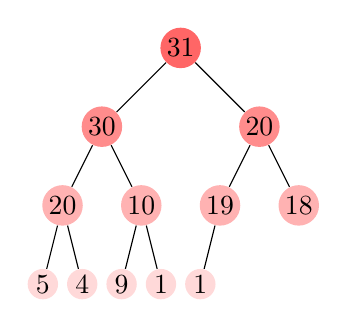
\begin{tikzpicture}[level distance=10mm]
	\tikzstyle{every node}=[fill=red!60,circle,inner sep=1pt]
	\tikzstyle{level 1}=[sibling distance=20mm,
	set style={{every node}+=[fill=red!45]}]
	\tikzstyle{level 2}=[sibling distance=10mm,
	set style={{every node}+=[fill=red!30]}]
	\tikzstyle{level 3}=[sibling distance=5mm,
	set style={{every node}+=[fill=red!15]}]
	\node {31}
	child {node {30}
		child {node {20}
			child {node {5}}
			child {node {4}}
		}
		child {node {10}
			child {node {9}}
			child {node {1}}
		}
	}
	child {node {20}
		child {node {19}
			child {node {1}}
			child[fill=none] {edge from parent[draw=none]}
		}
		child {node {18}}
	};
	\end{tikzpicture}
\end{frame}

\subsection{Subsection 1.2}
\begin{frame}{Example slide B}
	\begin{block}{Block 1}
	\begin{itemize}
	\item Bullet point 1 $x \in X$
	\pause
	\item Bullet point 2
	\item \dots
	\end{itemize}
	\end{block}
\end{frame}

\section{Section 2}
\begin{frame}{Example slide C}
	\begin{exampleblock}{Example 1}
	\begin{itemize}
	\item Bullet point 1
	\pause
	\item Bullet point 2
	\item \dots
	\end{itemize}
	\end{exampleblock}
\end{frame}

\begin{frame}{Example slide D}
	\begin{alertblock}{Alert 1}
	\begin{itemize}
	\item Bullet point 1
	\pause
	\item Bullet point 2
	\item \dots
	\end{itemize}
	\end{alertblock}
\end{frame}



\section{Suchen und Sortieren}
\subsection{Insertionsort}
\begin{frame}
\begin{algorithm}[H]
	\caption{Euclid’s algorithm}\label{euclid}
	\begin{algorithmic}[1]
		\Procedure{Euclid}{$a,b$}\Comment{The g.c.d. of a and b}
		\State $r\gets a\bmod b$
		\While{$r\not=0$}\Comment{We have the answer if r is 0}
		\State $a\gets b$
		\State $b\gets r$
		\State $r\gets a\bmod b$
		\EndWhile\label{euclidendwhile}
		\State \textbf{return} $b$\Comment{The gcd is b}
		\EndProcedure
	\end{algorithmic}
\end{algorithm}
\end{frame}


\appendix
\beginbackup

\begin{frame}[allowframebreaks]{References}
	\printbibliography
\end{frame}

\backupend

\end{document}
